%Chapter 2
\chapter{Review of the Literature}
\label{Chapter2}
%---------------------------------------------------------------------------------------
\section{No Free Lunch Theorem}
Introduced in Wolpert and Macready's ``No Free Lunch Theorems for Optimization''
1997 paper, the No Free Lunch theorem states that the performance of all
algorithms, when averaged out across all datasets, should be the same; that is
to say there is no one algorithm that is universally the best. The root cause of
this phenomenon is in that differing algorithms make different assumptions
about the distributions from which the data the algorithm's data arises. A
learning algorithm with an implicit assumption of a random distribution will
have a far lower test case classification accuracy than an algorithm that
assumes a Gaussian distribution if the distribution from which the set of
observed samples derive is truly normal and vice versa, if the
distribution is truly random, the Gaussian classifier's accuracy will suffer
relative to the classifier with a random assumption.
%------------------------------------------------------------------------------------
\section{On Meta Learning}
Before describing each of the individual meta learners compared within this
experiment, it is necessary to describe what a meta learning algorithm is.
Much like regular machine learning algorithms, meta learning algorithms use regularities
within processed inputs to make predictions on new instances (\textit{i.e} generalization).
Where meta learners differ from base learners is in the scope of the level of their adaptation; whereas
learning at the base level is focused on accumulating experience on a specific
learning task ($e.g.$, credit rating, medical diagnosis, mine-rock discrimination,
fraud detection, etc.), learning at the meta level is concerned with accumulating
experience on the performance of multiple applications of a learning system
\cite{Vilalta}. As such, base learners attempt to optimize performance with
respect to a specific task or problem domain, while meta learners attempt to
predict what the best base learner would be for a given task or problem domain.
This allows users wishing to use machine learning in their problem domain to skip
the struggle associated with discovering the best algorithm for the specific
problem; they need only gain access to a trained meta learner, present the dataset
they wish to analyze, then make use of the base learner suggested by the meta
learner.

All meta learners operate in two phases: Acquisition mode and advisory mode.
During the knowledge acquisition mode, the main goal is to learn about the
learning process itself \cite{Vilalta}. The meta learner receives as its input
during this phase a set of database sets (hereafter referred to as a ``metabase'')
from which dataset characteristics and run statistics are extracted. The goal
of the extraction of these characteristics and statistics is to gather
information that can be used to generalize the run results from this specific
metabase to other unprocessed distributions.

\begin{figure}[h]
\resizebox{\columnwidth}{!}{%
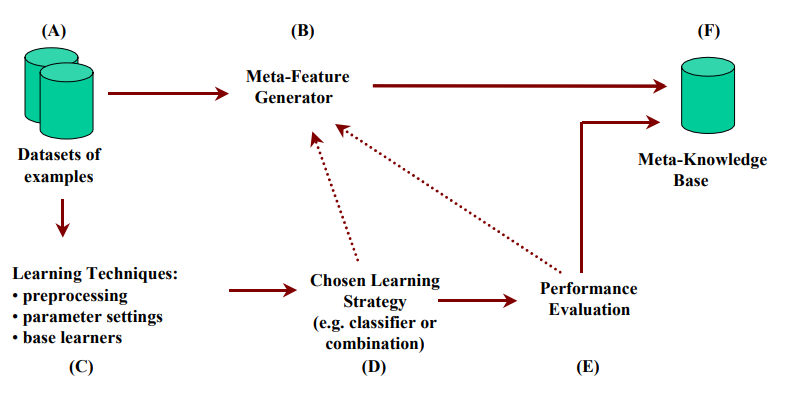
\includegraphics{Chapters/Images/MetaLearningAcquasition/MetaLearningAcquasition.PNG}}
\caption{An Example of Meta Learner Knowledge Acquisition}
\centering
Image borrowed from \cite{Vilalta} \\
Parameter setting not applicable in this experiment
\end{figure}

In advisory mode, the meta learning system makes use of the knowledge gathered in
the acquisition phase in order to suggest a best learning algorithm for a new
dataset. Meta features extracted from the dataset are ``matched'' with the
meta knowledge base to produce a recommendation regarding the best available
learning strategy \cite{Vilalta}.

What this entails is a mapping between meta features and an optimum base learning
strategy. In the case of this thesis, this mapping is accomplished via the $k$-means
algorithm, with the meta features being a set of standard statistical measures
in the case of the brute force and active strategies (these features are described
in section 3.3) and the meta features being ``learning curves'' in the case of the
curve comparison strategy (these curves are described in section 2.3.3).

\begin{figure}[h]
\resizebox{\columnwidth}{!}{%
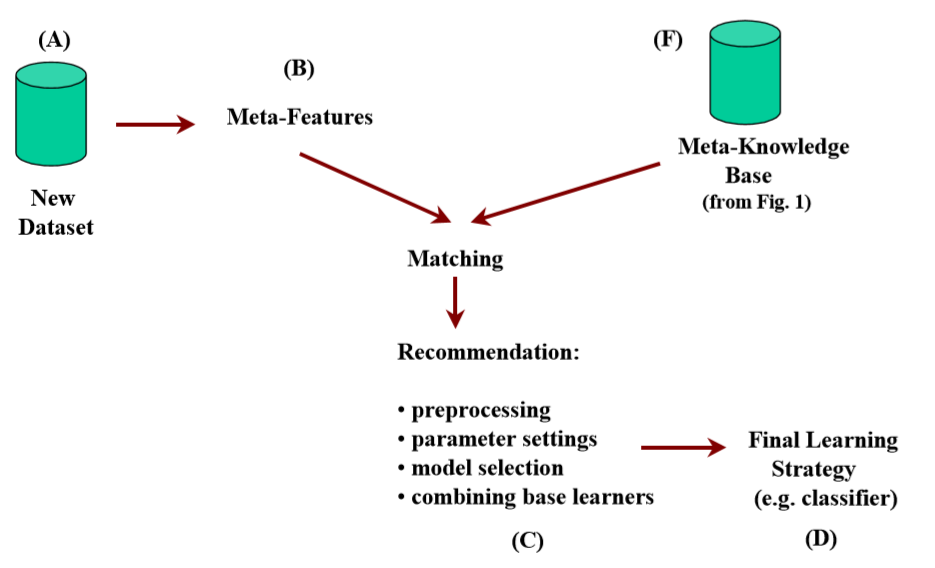
\includegraphics{Chapters/Images/MetaLearningAdvisory/MetaLearningAdvisory.PNG}
}
\caption{An Example of Meta Learner Advisory Mode}
\centering
Image borrowed from \cite{Vilalta} \\
Parameter setting not applicable in this experiment
\end{figure}

%-------------------------------------------------------------------------------------------
\section{Summary of the Compared Meta Learning Strategies}
In order to ascertain whether the NFL theorem applies to meta learning strategies,
we require a set of meta learning strategies with which to make run comparisons. The
meta learning strategies used in the experiment that comprises this thesis are described within
this section.
%-------------------------------------------------------------------------------------------
\subsection{Brute Force Metabase}
This is the most basic meta-machine learning algorithm. During the acquisition phase,  the
accuracies of the meta learner's producible machines for some metabase are gathered
and stored within a database. Classification of a new dataset $d_n$ during advisory
mode is accomplished via the usage of a clustering algorithm ($k$-Means in the case
of this experiment) and is used to find $d_m$, the dataset within the metabase
to which the new dataset $d_n$ is most similar. The algorithm which was found
to have had the greatest classification accuracy for the metabase dataset $d_m$
during acquisition will then be returned by the meta-learner.
\begin{figure}[h]
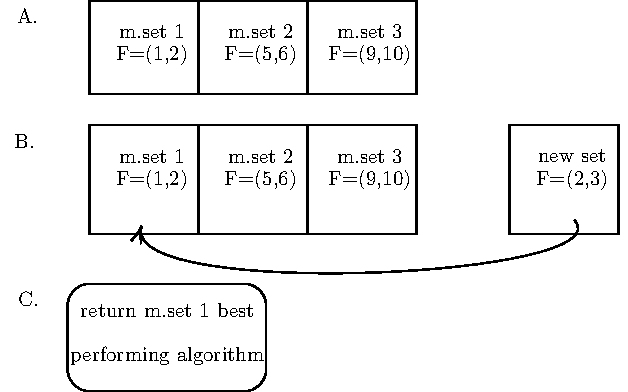
\includegraphics{Chapters/Images/BaseLearner/BaseLearner.pdf}
\caption{Example of base meta learning}
\centering
\begin{flushleft}
A. Metabase sets with given meta feature vectors \\
B. Classify new dataset by meta feature vector comparison \\
C. Return best algorithm of associated meta base set
\end{flushleft}
\end{figure}
%-------------------------------------------------------------------------------------------
\subsection{Active Meta Learning}
The second of the meta learning strategies implemented within this study, Active
Meta Learning is a meta learning technique  ``that reduces the cost of
generating Meta examples by selecting relevant Meta examples'' \cite{Bhatt}.
What this entails is a decision on what datasets to allow into a meta learner's
metabase during acquisition mode. Rather than analyze every candidate meta base
dataset, an active meta learner will analyze the next dataset with the highest
uncertainty. The relative uncertainty between two datasets is defined to be:
$$\delta(V_x,d_i,V_x,d_j) = \frac{|V_x,d_i - V_x,d_j|}{Max_{k\neq i}(V_x,d_k)- Min_{k\neq i}(V_x,d_k)},$$
where $V_x,d_k$ is the value of some meta parameter $V_x$ for dataset $d_k$,
$Max_{k\neq i}(V_x,d_k)$ is the maximum value of $V_x,d_k$ when dataset $i$ is
removed and $Min_{k\neq i}(V_x,d_k)$ is its corresponding minimum. Determining
which dataset has the overall highest uncertainty can be done via the following
procedure. First, sum the relative uncertainties for each dataset and
meta parameter combination. Then, rank the uncertainty scores of the datasets within
each meta parameter. After obtaining the uncertainty ranks within each parameter
for each dataset, sum the parameter ranks in order to obtain an overall
uncertainty rank for each dataset. Finally, select the parameter with the
highest rank for inclusion in the metabase. The equation representing the
overall uncertainty score in a specific meta parameter $V_x$ for dataset $d_i$ is
$$\delta(V_x,d_i) = \frac{\sum_{j\neq i} |V_x,d_i - V_x,d_j|}{Max_{k\neq i}(V_x,d_k)- Min_{k\neq i}(V_x,d_k)}.$$
\begin{figure}[h]
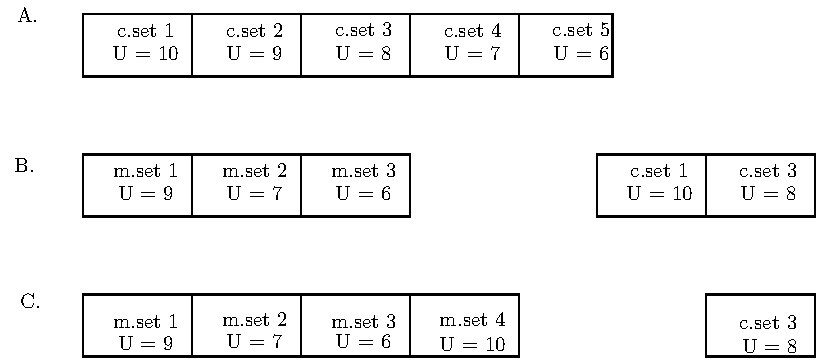
\includegraphics{Chapters/Images/ActiveLearner/ActiveLearner.pdf}
\caption{Example of active meta learning}
\centering
\begin{flushleft}
A. Set of candidate metabase sets \\
B. Random selection of half the original candidates \\
C. Inclusion of half remaining candidates by uncertainty comparison \\
\end{flushleft}
\end{figure}
%-----------------------------------------------------------------------------------------------
\subsection{Predicting Relative Performance of Classifiers from Samples}
Introduced in the paper ``Predicting Relative Performance of Classifiers from
Samples,'' the strategy of nearest learning curve comparison gathers run
statistics on the datasets within its metabase at various fractions of the full
size of the training portion of that dataset \cite{Leite}. It is then possible to plot a 2D
``learning curve,'' with the $x$ axis of such a graph being a specific fraction
of the training set and the $y$ axis of such a graph being the test classification
accuracy at that percent. The creation of these learning curves for each of the
datasets within the metabase is the work of this meta learning strategies
acquisition mode.

The categorization of new datasets during advisement mode can then be
accomplished in two steps. First, a model is trained on the new dataset with
some fractions of its training set using each candidate algorithm. These results
are then compared with the learning curves of each of the sets in the metabase.
The meta learner then returns the best algorithm of the dataset within the
metabase to which the new datasets learning curves is most similar. The
authors state that this process trains its meta learner in less time than a
brute force learner and that the resultant meta learner will also have a higher
classification accuracy than a brute force meta learner.

\begin{figure}[h]
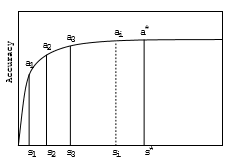
\includegraphics{Chapters/Images/LearningCurve/LearningCurve.PNG}
\caption{Example of a learning curve}
\centering
\begin{flushleft}
where: \\
A. Horizontal axis: Fractions of training set \\
B. Verticle axis: Test case accuracy for given set fraction \\
\end{flushleft}
Image borrowed from \cite{Leite}
\end{figure}
%----------------------------------------------------------------------------------------
\section{Summary of Producible Machines}
The strategies mentioned in the previous section all have advisory modes in which
a vector representation of an unprocessed dataset is consumed and a
prediction as to what algorithm would best be able to classify its data is made.
The machines that these strategies can choose from are the $k$-means clustering
algorithm, a neural network, a naive Bayes classifier, the support
vector machine, and regression. A brief description of each of these different
learning algorithms will comprise the rest of this chapter. For a more in-depth
discussion of the algorithms discussed within this chapter, the reader should consult
the appropriate chapter in Murphy's general purpose machine learning text
\cite{Murphy}.
%--------------------------------------------------------------------------------------------
\subsection{Linear Regression}
Linear regression is one of the most common and oldest machine learning
techniques. It asserts that the response is a linear function
of the inputs \cite{Murphy}. This relation takes the following form:
$$ y(\textbf{x}) = \textbf{w}^T\textbf{x} + \epsilon = \sum_{j=1}^{D}w_jx_j + \epsilon,$$
where $\textbf{w}^T\textbf{x}$ represents the inner or scalar product between the input vector $x$
and the model's weight vector $\textbf{w}^T$, and $\epsilon$ is the residual error
between our linear predictions and the true response.

To fit a linear regression model, the least squares approach is usually used.
Given some  ``overdetermined'' linear system (that is to say a system in which
there are more data points than parameters), one can write an expression for the
sum of squares of the system
$$S(\beta) = (y_1 - \beta x_1)^2 + (y_2 - \beta x_2)^2 + ... (y_n - \beta x_n)^n,$$
and then take the partial derivative of this sum of squares deviations with respect
to each of the components of $\beta$, set them to zero, then solve the resulting
equations to directly determine the values of the parameters that
minimize the sum of the squared errors of the system. With linear regression in
two dimensions (one dimension in the Independent variable and one dimension in
the Dependent variable, we see a system with two parameters:
$\beta_0 = y~intercept$ and $\beta_1 = slope$. If we had, for example, 3 data
points (2,1),(3,7), and (4,5) we would have the equations
$\beta_0 + 2*\beta_1 = 1$, $\beta_0 + 3*\beta_1 = 7$, and
$\beta_0 + 4*\beta_1 = 5$. The sum of squared errors would then be
 $S(\beta_0,\beta_1)= [1 - (\beta_0 + 2*\beta_1)]^2 + [7 - (\beta_0 + 3*\beta_1)]^2 + [5 - (\beta_0 + 4*\beta_1)]^2$
, which we could then differentiate with respect to $\beta_0$ and $\beta_1$, then
directly solve the resulting set of linear equations for the minimum of
the summed squares.
%--------------------------------------------------------------------------------------------
\subsection{Naive Bayes}
The Na\"{i}ve Bayes classifier algorithm uses Bayes rule to construct a classifier
that makes a simplifying assumption. Given a set of discrete-valued
features $x \in {1,...,K}^D$, we can calculate the class conditional density for
each feature, then, with our assumption of independence, generate a guess
at what the class should be for a new input, by multiplying the conditional
likelihood values for each of the new inputs features times the prior on the
desired to be known class, that is to say
$p(y|\textbf{x}) \propto p(y) \sum_{j}^{D}p(x_j|y)$.
The calculation of the posterior probability for a new example can be done
manually, or can be derived from distributions that are inferred from the
provided data. Consider, for example, a collection of data listing individuals
that did or did not purchase a house from a real estate agent, where, for some
reason or another, the only data remaining pertaining to these individuals are:
what their income level was, what their age was, and how far they have to or
would have had to drive to work from their new home.

Say, for example, we get a new datapoint: income: \$25,000, age: 30, distance: 10. In this
case the conditional likelihood of this data given a yes for each of the
individual features is 2/9, 1/9, and 2/9 respectively. The prior on yes is 1/3.
The marginal likelihoods of each of the individual features are 2/9, 1/9 and 2/9
respectively. As such, the posteriors for our new datapoint are
$p(y=yes|x)=\frac{(2/9)*(1/9)*(2/9)*(9/27)}{(6/27)*(3/27)*(6/27)} = \frac{0.00182}{0.00548} = 0.33$ and $p(y=no|x)=\frac{(4/18)(2/18)(4/18)(18/27)}{(6/27)(3/27)(6/27)} = \frac{0.0036}{0.00548} = 0.66$.

Note that $0.66 > 0.33$ and as such our classifier would label this datapoint
with a no, this individual is not likely to purchase a house.

%--------------------------------------------------------------------------------------------
\subsection{Support Vector Machine}
The support vector machine (SVM) is a binary classification algorithm that
attempts to find a hyperplane that separates the inputs within a given input
space with a maximum margin of separation between the hyperplane and the
``support vectors,'' those vectors on either side of the hyperplane
that are closest to it. To arrive at a form of the support vector machine that
can be used to classify new inputs, one first needs a representation of the
potential separating hyperplane $$y_i(\mathbf{w}*\mathbf{x}_i + b) > 1,$$ where
$y_i$ is the truth label of given training input $\bold{x}_i$, $\bold{w}$ is a vector
normal to our candidate separating hyperplane that represents how much
``weight'' is to be applied to an input, and $b$ is a bias constant representing
the threshold the weight/input product needs to pass before it is considered
classified. The distance of a given hyperplane can be determined by calculating
the difference between these previously mentioned ``support vectors'' in the
direction normal to this hyperplane. This difference can be calculated via the
following equation:
$$(\bold{x_{s+}}-\bold{x_{s-}})\bold{\frac{w}{||w||}},$$ where $\bold{x_{s+}}$
and $\bold{x_{s-}}$ are respectively positive and negative support vectors and
$\bold{\frac{w}{||w||}}$ is the unit vector in the direction normal to the hyper
plane towards the positive examples. The size of the margin is $2/||w||$. As
such, the discovery of a working SVM can be accomplished by solving a constrained
optimization problem in which the thing to be minimized is $1/2||w||^2$, subject
to the constraints $y_i(\bold{w}*\bold{x_i} + b) = 1$ for support vectors.
Crafting an expression of this constrained optimization that can be solved by a
computer can be done by taking the Lagrangian:
$$L(\bold{W},\bold{\lambda},\bold{Y}) = 1/2||\bold{w}||^2 \sum_{i=1}^{n}y_i(\bold{w}*\bold{x_i}+b)-1,$$
then taking care of the fact that the vector $w_o$ that determines the optimal
hyperplane can be written as a linear combination of the training vectors:
$w_{0}=\sum_{i=1}^{n}y_{i}\alpha_{i}^{0}\bold{x_i}$ \cite{Vapnik}. Swapping this
equation into the Lagrangian yields:
$$L = \sum \alpha_{i} - 1/2 \sum_{i}\sum_{j}\alpha_{i}\alpha_{j}y_{i}y_{j}(\bold{x_i}\cdot\bold{x_j}),$$
which can be optimized computationally.

This final form of the Lagrangian reveals the support vector machine's most
powerful attribute: the kernel. The optimization of the hyperplane within the
inputs depends only on the dot product of pairs of inputs; they do not appear
anywhere else in the Lagrangian other than the very end and then only so as
pairs of dot products. This fact allows the writing of a decision function on
new inputs: $$f(\bold{u}) = \sum_{i}^{N}\alpha_{i}y_{i}(\bold{x_i}\cdot\bold{u})+b,$$
where $\bold{u}$ is a vector whose label we do not know. The support vector
machine can use kernels to map input vectors into
non-linear high-dimensional feature space without actually calculating the
position of the vectors within that feature space \cite{Vapnik}. The kernel
accomplishes this by calculating the distance (or similarity)between two
input vectors in this space without reference to their exact position within
this higher space. This then allows the computation of a linear separation
between the points in this higher dimensional space which translates into a
non-linear separation for the vectors in their original lower dimensional space
where a separation might otherwise not have been discoverable.
%--------------------------------------------------------------------------------------------
\subsection{$k$-Means Clustering}
The objective of the $k$-means algorithm is to partition a dataset into k groups
such that the points within some group are all closer to
the mean of that group than they are to any other group. A clear
informal explanation of the work that the $k$-means algorithm performs
was given by James MacQueen in 1967: ``...the $k$-means procedure
consists of simply starting with k groups each of which consists of a
single random point, and thereafter adding each new point to the
group whose mean the new point is nearest. After a point is added to
a group, the mean of that group is adjusted in order to take account
of the new point. Thus at each stage the $k$-means are, in fact, the
means of the groups they represent'' \cite{MacQueen}. Formally stated,
given an integer $k$ and a set of $n$ data points in
$\mathbb{R}^{d}$ the $k$-means algorithm seeks to minimize $\Phi$, the
over all total summed in class distance between each point and its
closest center such that $\Phi = \sum_{x \in X} min_{c \in C}||{x-c^{2}}||$
\cite{Arthur}.

The $k$-means model is a type of Gaussian mixture model that is trained with a
procedure called expectation maximization. Given a set of distributions with
missing data, mixture models tend to have derivatives that are either difficult
to define or are entirely undefinable. On the other hand, the calculation of some
ML/MAP (maximum likelihood/maximum a posteriori) estimates for some set of models
can generally be done with little difficulty if every point within the
distributions is known (at which point our learner would have nothing to do) and
thus calculus would be unnecessary ($i.e.$, it would not matter that the derivative
cannot be defined). Expectation maximization uses this fact in order to obtain an
estimation of the ML/MAP indirectly. The algorithm consists of two steps. First,
an estimate as to what the expected value of the hidden data is based off the
current guess for the parameters is made. Then, the likelihood function for the
parameters is maximized under the assumption that the data discovered in the
previous step are complete, $i.e.$, that there are no longer any hidden data. These
steps are then repeated until some convergence criterion is met. The $k$-means is
exactly this type of algorithm, but with the covariance matrix
$\Sigma_{k} = \rho^{2}*I_{D}$ and the mixing weights $\Pi_{k} = 1/K$ all being fixed,
such that the only free parameters are the cluster centers $\mu_{k} \in \mathbb{R}^{D}$,
and such that the hidden data is the ground truth label of the data points.
%--------------------------------------------------------------------------------------------
\subsection{Neural Network}
A neural network is a type of machine learning algorithm that mimics
the inter-connectivity of animal brains in order to automatically
discover rules to classify given inputs. The neural network is one of the most
flexible learning algorithms within literature, so flexible in fact that it is
capable of approximating any continuous function \cite{Hornik}. As such, its
inclusion within a meta learning system is almost mandatory.  Generally,
a neural network system works by first being presented with a set of classified or
unclassified inputs. Said system will then attempt to
make a decision on these inputs on which an error value will then be
assigned. The system will then see some kind of correction function
applied to it. This process will continue until the system has
exhausted its supply of training data, at which point it will
hopefully have discovered a strong set of rules for performing whatever
work it is that it was designed to perform.

The type of neural network that will be used within this thesis is
what is called the feed-forward neural network (a.k.a. multilayer perceptron,
or MLP). The feed forward neural network is essentially a series of
logistic regression models stacked on top of each other, with the
final layer being either another logistic regression or linear
regression model depending on whether or not a classification or
regression problem is being solved \cite{Murphy}. The leftmost
layer of this stack is called the input layer and consists of a set of
neurons ${x_i|x_1,x_2,x_3,...,x_m}$ representing the input's
features. Each neuron in the hidden layer transforms the values from
the previous layer via weighted linear summation $w_1x_1 + w_2x_2 +...+w_mx_m$
which is then passed into a non-linear action function $g()$, such as the
logistic function or the hyperbolic tangent function. It is important to note
that $g$ must be non-linear, otherwise the entire model will collapse into a
large linear regression model of the form $y = w^T(Vx)$ \cite{Murphy}.

The multi-layer perceptrons created in this experiment will be trained
by an error propagation/training technique called backpropagation.
Backpropagation is a procedure that repeatedly adjusts the weights of the
connections in a neural network so as to minimize a measure of the difference
between the actual output vector of the net and the desired output
vector \cite{Rumelhart}. In order to accomplish this, the algorithm
adjusts the weights of the neural network by considering the error of
the outputs then minimizes this error via gradient descent with respect
to each of the weights within the network. Specifically, the gradient
vector of the negative log-likelihood error on the output neurons is
computed by use of the chain rule of calculus \cite{Murphy}. Say we
have a one layer neural network in which the hidden layer is described
by $\alpha^{L} = \sigma(w^{L}\alpha^{L-1} + b^{L}) = \sigma(z^{L})$,
where $L$ superscript refers to the hidden layer and $L-1$ refers
to the input layer of the network. The parameters of this network can
be said to be $\Theta = (V,W)$ where $V$ is the weight vector for the input
layer and $W$ is the weight vector for the hidden layer. The error (or
more specifically the costs function) of a such a network is given by:
$$J(\Theta ) = - \sum_n\sum_k(\hat{y}_{nk}(\Theta)-y_{nk})^2$$
in the case of regression, and via cross-entropy,
$$J(\Theta ) = - \sum_n\sum_ky_{nk}log\hat{y}_{nk}(\Theta),$$
in the case of classification. The gradient of this error $\nabla_{\Theta}J$
is found via the chain rule of calculus:
$$\frac{\partial C}{\partial
w^{L}} = \frac{\partial z^{L}}{\partial
w^{L}}\frac{\partial \alpha}{\partial z^{L}}\frac{\partial
  C}{\partial \alpha^{L}}.$$
This equation is easiest to understand if read from right to left.
Notice how in each stage the rates being compared are between nearest
elements, first the error to the output that produced it, then the output
to the element to which the non-linearity is applied, then finally the the
non-linearity receiving value to the weight vector. The result of this
calculation easily gives us the direction of the gradient, the negative of
which we will use to modify $w^{L}$ in a direction that will reduce the output
error. Reduction of the error of a multilayer perceptron with more
than one neuron in each layer works mostly the same way. Once again,
the chain rule of calculus is used in order to find the derivative of
the output error with respect to the weights of the connections
between the hidden layer before the output neurons and the output
neurons $\frac{\partial C}{\partial w^{L}_{n-j}}$, where $L$ is the
target neuron's layer (the last layer in this case), $n$ is the index of
a neuron within this layer, and $j$ is the index of the neuron in the
previous layer $L-1$ from which neuron $n$ is receiving input (note
that in this case the hyphen does not mean subtract, but rather
indicates that there is a connection between these neurons). For an output
neuron, its error is then given by:
$$\frac{\partial C}{\partial w^{L}_{n-j}} = \frac{\partial z^{L}_{j}}{\partial w^{L}_{n-j}}\frac{\partial \alpha^{L}_{j}}{\partial z^{L}_{j}}\frac{\partial C}{\partial \alpha^{L}_{j}},$$
with the error relative to neurons earlier in the network being calculable by
continuing usage of the chain rule.

%For an excellent and intuitive explanation of how neural networks work,
%pls consider viewing the animated overview of the method at 3Blue1Brown's
%youtube channel.
% WAY TOO INFORMAL!
